\documentclass[a4paper]{article}

\usepackage[english]{babel}
\usepackage[utf8x]{inputenc}
\usepackage{amsmath}
\usepackage{graphicx}
\usepackage[colorinlistoftodos]{todonotes}
\PassOptionsToPackage{hyphens}{url}\usepackage[colorlinks=true,urlcolor=blue]{hyperref}
\urlstyle{same}
\sloppy

\title{AMORO Lab - Part 1: Introduction}
\author{Damien SIX \\ damien.six@ls2n.fr}
\date{Released: August 18, 2021}

\begin{document}
\maketitle

\section{Objectives of the lab}

The purpose of this lab is to perform the simulation of two parallel robots using ROS2 and GAZEBO. For each robot, you will compute the kinematic and dynamic models and compare them to the simulator output. Then, you will develop a computed torque control for the simulator.

Two robots will be simulated: a five-bar mechanism and a biglide mechanism. For the five-bar, the models are already available in your course and a reminder is provided with the content of this lab. For the biglide, in addition to the simulation, you have to perform and report the computation of the several models.

\textbf{All the reports for this lab have to be done using \LaTeX. Templates are provided in the lab content.}
If you have no knowledge of what is \LaTeX, please refer to the \href{https://www.latex-project.org/about/}{the official documentation}, the documents provided and your lab supervisor.

There is no lab report on the first part of the lab (five-bar mechanism). However, your work on the second mechanism (biglide) have to be fully reported. 

\section{Gazebo and ROS2}
The simulation for this lab is performed by \href{http://gazebosim.org/}{Gazebo}.  \href{https://docs.ros.org/en/foxy/index.html}{ROS2} topics are used to communicate with the simulation, providing torque inputs and getting measures (joints, end effector) from the simulation.

\begin{figure}
    \centering
    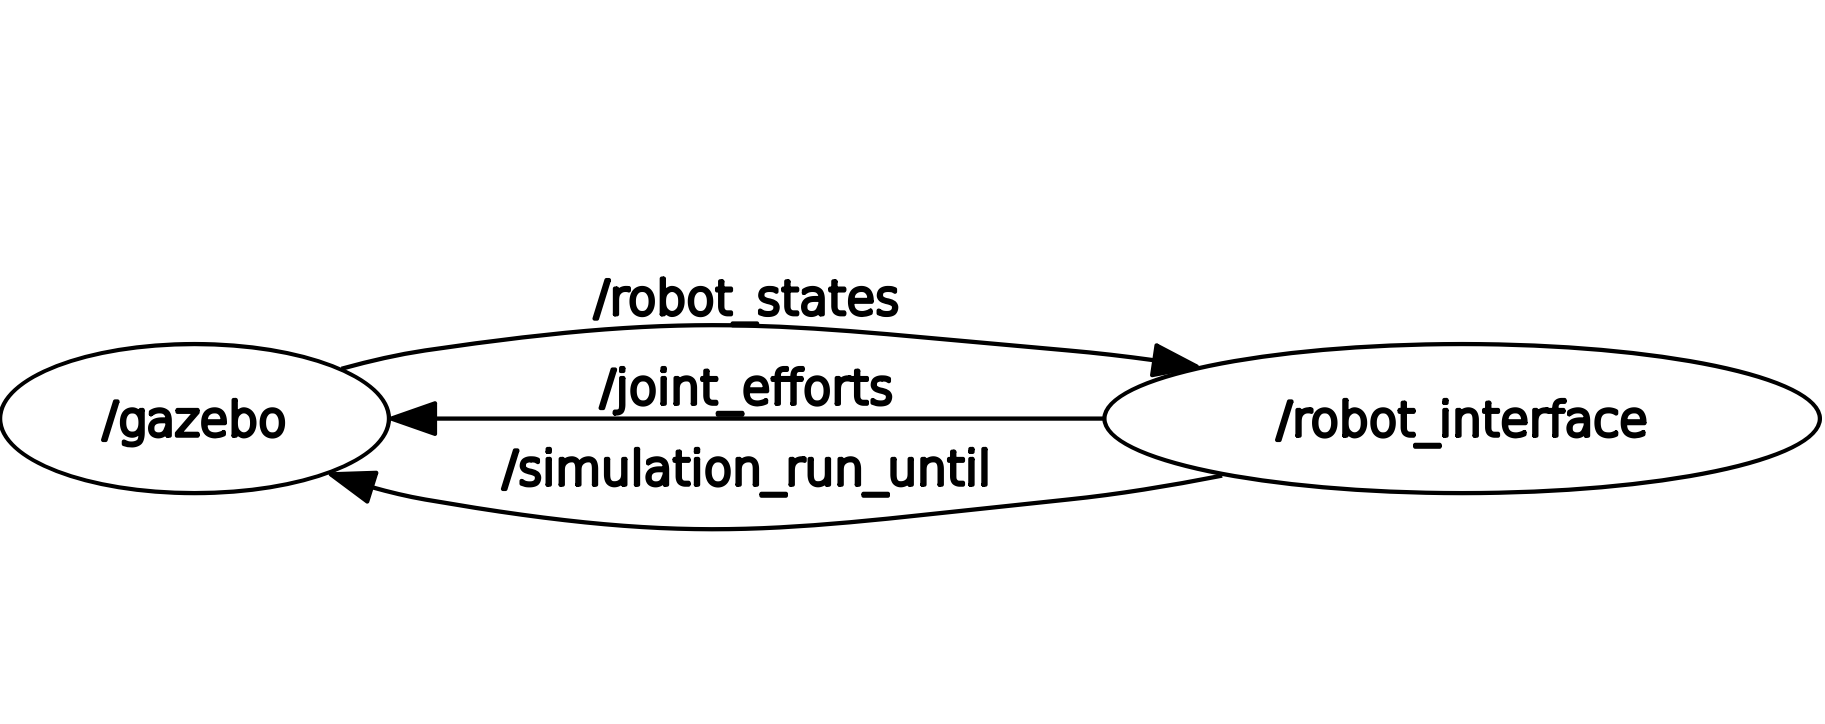
\includegraphics[width =\textwidth]{ros2_nodes.png}
    \caption{ROS2 nodes for the robot simulation}
    \label{fig:nodes}
\end{figure}

For the purpose of this lab, ROS2 and communication with Gazebo is hidden via a Python class Robot. In the scripts you will write, you can interact with the robot using
\begin{itemize}
    \item \textit{robot.start\_oscillate()} to perform some oscillations on the robot joint (usefull to test models without predefined trajectory). You can also stop oscillations using \textit{robot.stop\_oscillate()}. 
    \item \textit{robot.active\_left\_joint.position} to access the position of the left active joint of the robot. Similarly, you can access any joint (passive/active, left/right) and several data (position/velocity/acceleration/effort). 
    \item You can also access the end effector data using 
    \textit{robot.end\_effector.position\_x} for the x coordinate of the end effector. You can also access the y coordinate and velocity/acceleration data.
    \item You can set some joint efforts using 
    \textit{robot.apply\_efforts(left\_joint, right\_joint)}. Indeed, the robot should not be in oscillate mode for this to work properly.
    \item \textit{robot.get\_time()} to get the current simulation time. Useful to plot curves.
\end{itemize}
% 
The simulation is performed in a way that Gazebo is driven by the Robot class. Each time you send a torque input, the simulation will perform a 10~ms simulation then send you back the results. The normal way to control the simulation is
\begin{itemize}
    \item Send a torque input using \textit{robot.apply\_efforts()} or \textit{robot.continue\_oscillations()} in oscillation mode.
    \item Wait for the results of Gazebo simulation. This is checked using \textit{robot.data\_updated()}.
    \item Do whatever you need to do.
    \item Send a new torque input.
    \item Loop as long as you need.
\end{itemize}
%
Scripts are already pre-filled to help you with this part.
%
\section{Prepare for the lab}
To prepare the lab, the following steps must be performed.
\begin{itemize}
	\item Switch to ros2 by typing \textit{ros2ws}.
    \item Create a \textit{ros2} folder and a \textit{src} sub-folder in it.
    \item Clone the lab folder into the \textit{ros2/src} folder using the command\\
        \$ git clone https://gitlab.univ-nantes.fr/six-d-1/lab\_amoro\\
    \item Compile and install everything using the command \textit{colbuild}.
    \item Test the correct installation using \textit{ros2 launch lab\_amoro gazebo.launch.py}\\
    If Gazebo is launched after typing this command, you are ready to go.
\end{itemize}
When you open a new terminal, you must always type the command \textit{ros2ws} to work under ros2 (otherwise it is ros1 by default).
\end{document}